\documentclass{article}

\usepackage{fullpage}

\usepackage{amsmath}
\usepackage{amssymb}
\usepackage{graphicx}
\usepackage[colorlinks,linkcolor=dblue,filecolor=black,citecolor=dblue,urlcolor=dblue]{hyperref}
\usepackage{etex}
\bibliographystyle{alpha}
\usepackage[english]{babel}
\usepackage{amsfonts,amssymb,amsmath,sectsty,url}
\usepackage{mathrsfs}

\usepackage{tikz}
\usetikzlibrary{calc}
\usepackage{color}
%\usepackage{mathtools}
\usepackage[all]{xy}
\usepackage{ctable}
% \usetikzlibrary{calc}

\usepackage{graphicx}
\usepackage{ifpdf}
\usepackage{multirow}
\usepackage{multicol,color}
\usepackage{tablefootnote}


\usepackage{amsthm}

\theoremstyle{plain}
\newtheorem{theorem}{Theorem}[section]
\newtheorem{corollary}[theorem]{Corollary}
\newtheorem{lemma}[theorem]{Lemma}%[section]
\newtheorem{proposition}[theorem]{Proposition}%[section]

\theoremstyle{definition}
\newtheorem{definition}[theorem]{Definition}
\newtheorem{example}[theorem]{Example}%[section]
\newtheorem{construction}[theorem]{Construction}


\theoremstyle{remark}
\newtheorem{remark}[theorem]{Remark}
\newtheorem{fact}[theorem]{Fact}%[section]
\newtheorem{observation}[theorem]{Observation}
\newtheorem{claim}[theorem]{Claim}%[section]



% COMMANDS

\renewcommand{\emptyset}{\varnothing}

% Colors

\definecolor{dblue}{rgb}{0.00, 0.50, 0.90}
\definecolor{lblue}{rgb}{0.70, 0.80, 1.00}
\definecolor{lpink}{rgb}{0.90, 0.70, 1.00}
\definecolor{lgreen}{rgb}{0.80, 0.95, 0.75}
\definecolor{lred}{rgb}{0.99, 0.50, 0.55}
\definecolor{lyellow}{rgb}{1.00, 0.95, 0.75}
\definecolor{llgrey}{rgb}{0.95, 0.95, 0.95}
\definecolor{salmon}{rgb}{0.99, 0.90, 0.90}

% UC security things

\newcommand{\secs}{\mathsf{aggregation}}
\newcommand{\Pss}{\Pi_\secs}
\newcommand{\Fss}{\mathcal F_\secs}
\newcommand{\Sss}{\mathcal S_\secs}


\newcommand{\elect}{\mathsf{election}}
\newcommand{\Pelect}{\Pi_\elect}
\newcommand{\Felect}{\mathcal F_\elect}
\newcommand{\Select}{\mathcal S_\elect}

\newcommand{\Commit}{\mathsf{Commit}}
\newcommand{\Open}{\mathsf{Open}}
\newcommand{\Pcomm}{\Pi_\Commit}
\newcommand{\Fcomm}{\mathcal F_\Commit}
\newcommand{\Scomm}{\mathcal S_\Commit}

\newcommand{\Fnoisegen}{\mathcal{F}_{\mathsf{noise}}}
\newcommand{\Pdpa}{\Pi_{\mathsf{dp}\textrm{-}\mathsf{aggregation}}}
\newcommand{\Pbinomial}{\Pi_\mathsf{binomial}}
\newcommand{\Pgauss}{\Pi_\mathsf{gauss}}
\newcommand{\Pfirstlaplace}{\Pi_\mathsf{laplace1}}
\newcommand{\Psecondlaplace}{\Pi_\mathsf{laplace2}}
\newcommand{\Ppack}{\Pi_\mathsf{pack}}


% CS things
\newcommand{\Oh}{ \mathcal{O} }
\newcommand{\QuasiOh}{ \widetilde{ \mathcal{O} } }

%\newcommand{\B}			{\mathrm{B}}
\newcommand{\KB}		{\mathrm{KB}}
\newcommand{\MB}		{\mathrm{MB}}
\newcommand{\GB}		{\mathrm{GB}}

\newcommand{\ms}		{\mathrm{ms}}
\newcommand{\mus}		{\mathrm{{\mu}s}}

% FE
\newcommand{\FE}{\mathsf{FE}} % FE
\renewcommand{\sec}{\lambda} % sec param
\newcommand{\PP}{\mathsf{PP}} % public parameters for FE
\newcommand{\MK}{\mathsf{MK}} % master secret key for FE
\newcommand{\Key}{\mathsf{Key}} % enc/dec secret key for (secret-key) FE
\newcommand{\Ctxt}{\mathsf{Ctxt}} % enc/dec secret key for (secret-key) FE

\renewcommand{\sf}{\mathsf{sf}} % semi-functional flag
\newcommand{\f}{\mathsf{f}} % functional flag


% Encodings
\newcommand{\A}{\mathbf{A}} % matrix for encoding
\renewcommand{\S}{\mathbf{S}} % secret matrix (tensored)
\newcommand{\B}{\mathbf{B}} % BP matrix
\newcommand{\E}{\mathbf{E}} % error matrix
\newcommand{\Y}{\mathbf{Y}} % result encoding matrix
\newcommand{\D}{\mathbf{D}} % trapdoor'd matrix
\newcommand{\J}{\mathbf{J}} % left bookend

\newcommand{\TrapSam}{\mathsf{TrapSam}}
\newcommand{\PreimgSam}{\mathsf{PreimgSam}}



% Sets, fields, rings, groups, etc...
\newcommand{\Id}{\mathbb{I}} % the identity matrix
\newcommand{\Z}{\mathbb{Z}} % the integers
\newcommand{\N}{\mathbb{N}} % the non-negative integers
\newcommand{\F}{\mathbb{F}} % a finite field
\newcommand{\K}{\mathbb{K}} % a finite field
\newcommand{\Kbot}{\mathbb{K}_{\bot}} % a finite field extended with bottom

\renewcommand{\P}{\{1,\dots,n\}} % player set $\{1,\dots,n\}$

%\newcommand{\K}{\mathcal{K}} % key space
\newcommand{\M}{\mathcal{M}} % message space
\newcommand{\T}{\mathcal{T}} % tag space
\newcommand{\R}{\mathcal{R}} % randomness space

\newcommand{\tensor}{\otimes}
\newcommand{\unit}{\mathbf{u}}
\newcommand{\transpose}[1]{#1^{\intercal}}
\newcommand{\identitymatrix}{\mathbb{I}}
%\newcommand{\identitymatrix}{\mathbb{1}}  % requires the bbold package
%\newcommand{\cartesian}[1]{{\times #1}}
\newcommand{\cartesian}[1]{{\times \! #1}}
%\newcommand{\cprod}{\bigtimes}  % requires the mathabx package



% Probability and DP
\newcommand{\Avg}{\textup{E}} % Average of random variables

\newcommand{\mechanism}[1]{\mathcal{ #1 }}
\newcommand{\norm}[1]				{\left\lVert #1 \right\rVert}
\newcommand{\e}	[1]						{\mathbf{e}^{#1}}
%\newcommand{\e}	[1]						{\mathrm{exp}(#1)}
\newcommand{\sensitivity}[2]		{\Delta_{#1} #2}
\newcommand{\intype}					{\mathcal{X}}
\newcommand{\dstype}					{\N^{\intype}}
\newcommand{\ds}						{D}

\newcommand{\given}			{\; | \;}
\newcommand{\condpr}[2]		{\pr{#1 \given #2}}
\newcommand{\distsOver}[1]		{\Delta #1}

%\newcommand{\hammingweight}[1]	{\mathrm{H}(#1)}
\newcommand{\hammingweight}[1]	{\mathrm{w_H}(#1)}

%\newcommand{\D}{\mathcal{D}} % a distribution
\newcommand{\U}{\mathcal{U}} % the uniform distribution

\newcommand{\coin}						{\mathcal{C}}
\newcommand{\uniform}[1]			{\mathcal{U}(#1)}
\newcommand{\binomial}[1]			{\mathcal{B}(#1)}
\newcommand{\gaussian}[1]			{\mathcal{N}(#1)}
\newcommand{\laplacian}[1]			{\mathrm{Lap}(#1)}
\newcommand{\distribution}			{\mathcal{D}}
\newcommand{\leftovernoise}		{\mathcal{E}}

\newcommand{\pr}[1]					{\Pr \left[ #1 \right]}
\newcommand{\floor}[1]					{\lfloor#1\rfloor}
\newcommand{\ceil}[1]					{\left\lceil#1\right\rceil}



% Labels

\newcommand{\pk}{\mathsf{pk}}
\newcommand{\sk}{\mathsf{sk}}


\newcommand{\off}{\texttt{off}}

\newcommand{\Sim}{\mathcal{S}}



% Operators

\newcommand{\AND}{\wedge}
\newcommand{\OR}{\vee}
\newcommand{\bigAND}{\bigwedge}
\newcommand{\bigOR}{\bigvee}

\newcommand{\asn}{\gets} % to be read as ``computed as'' or ``taken according to the distribution...'' or ``taken uniformly from...''

\newcommand{\ParamGen}{\mathsf{ParamGen}}
\newcommand{\Setup}{\mathsf{Setup}}
\newcommand{\KeyGen}{\mathsf{KeyGen}}
\newcommand{\Enc}{\mathsf{Enc}}
\newcommand{\Dec}{\mathsf{Dec}}
\newcommand{\Add}{\mathsf{Add}}
\newcommand{\ek}{ek}
\newcommand{\dk}{dk}
\newcommand{\plaintext}{m}
\newcommand{\ciphertext}{e}
\newcommand{\plaintextspace}{\mathcal{P}}
\newcommand{\ciphertextspace}{\mathcal{E}}
\newcommand{\INDCPA}{\textrm{IND-CPA}}

\newcommand{\Share}{\mathsf{Share}}
\newcommand{\SimShare}{\mathsf{SimShare}}
\newcommand{\Shamir}{\mathsf{Shamir}}
\newcommand{\PackedShamir}{\mathsf{PackedShamir}}
\newcommand{\RS}{\mathsf{RS}}
\newcommand{\Rec}{\mathsf{Recon}}
\newcommand{\SSS}{\mathsf{SSS}}

\newcommand{\share}{\sigma}
\newcommand{\secret}{m}

\newcommand{\MAC}{\mathsf{MAC}}
\newcommand{\Encode}{\mathsf{Encode}}


\newcommand{\Adv}{\mathsf{Adv}}
\newcommand{\Gen}{\mathsf{Gen}}
\newcommand{\AExpm}{\mathsf{Exp}}



\newcommand{\ineff}{\mathsf{ineff}}
\newcommand{\superpoly}{\mathsf{superpoly}}
\newcommand{\poly}{\mathsf{poly}}
\newcommand{\negl}{\mathsf{negl}}
\newcommand{\const}{\mathsf{const}}
\newcommand{\polylog}{\mathsf{polylog}}

\newcommand{\normtwo}[1]{\|{#1}\|_2}
\newcommand{\normI}[1]{\|{#1}\|_\infty}



% Environments
\newenvironment{boxfig}[2]{% {#1}{#2} = {Caption}{label}
\begin{figure}[ht!]
  \newcommand{\FigCaption}{#1}
  \newcommand{\FigLabel}{#2}
  \vspace{-\medskipamount}
  \begin{center}
    \begin{small}
      \begin{tabular}{@{}|@{~~}l@{~~}|@{}}
        \hline
        \rule[-1.5ex]{0pt}{1ex}
        \begin{minipage}[b]{.96\linewidth}
          \vspace{1ex}
          \smallskip
          }{%
        \end{minipage}\\
        \hline
      \end{tabular}
    \end{small}
    \vspace{-1\bigskipamount}
  \end{center}
    \caption{\small \FigCaption}
    \label{\FigLabel}
%  \vspace{-0.3cm}
\end{figure}
}



% LATEX

% this crossreferences description items
\makeatletter
\let\orgdescriptionlabel\descriptionlabel
\renewcommand*{\descriptionlabel}[1]{%
  \let\orglabel\label
  \let\label\@gobble
  \phantomsection
  \edef\@currentlabel{#1}%
  %\edef\@currentlabelname{#1}%
  \let\label\orglabel
  \orgdescriptionlabel{#1}%
}
\makeatother




% a temporary counter
\newcounter{tempcount}



\newcommand{\mr}[1]{{\textcolor{lblue}{\textbf{Mariana:} #1}}}
\newcommand{\vc}[1]{{\textcolor{lred}{\textbf{Valerie:} #1}}}
\newcommand{\vp}[1]{{\textcolor{dblue}{\textbf{Valerio:} #1}}}

\title{Multiparty Linear Regression via SPDZ}
\author{Valerie Chen \and Valerio Pastro \and Mariana Raykova}


\begin{document}

\titlepage
\maketitle

\pagebreak

\section{Preliminaries}
\vp{stuff}

\section{Experiments}
The experiments were run on the SPDZ framework, using a 128 bit and 256 bit prime field respectively. In the 128 bit prime field, the bits were allotted with 28 bits after the decimal place to match the 32 bit example in the original paper and 60 bits after the decimal for the original 64 bit case. Compared original paper, we needed more space to the left of the decimal for comparison purposes and operations using the fixed point type. However, we believe this is still a fair comparison because we are not working with more precision after the decimal place and if anything using more bits should actually slow down our calculations. For each generated matrix of varying dimensions, the features were split evenly between two parties. We then wanted to see if linear decomposition algorithms like LDLT, Cholesky, and CGD (with 5, 10, 15, and 20 iterations) were able to get comparable if not better results. 

First, we ran the two algorithms two gauge time and error rates for matrices of size 10, 20, 50, 100, 200, and 500, with 200000 features each. Secondly, we ran on a size 20 matrices with condition numbers varying from 1 to 10. Both parts were completed for both bit sizes to evaluate performance differences. To model after the original experiment, we ran iterations of 5, 10, 15, and 20 for the CGD algorithm but added on as an extension of 25 iterations to see if necessary (i.e. the errors were not comparable for all sizes or condition numbers), there was still room for improvement. 

\section{Result}

\begin{figure}[h]
  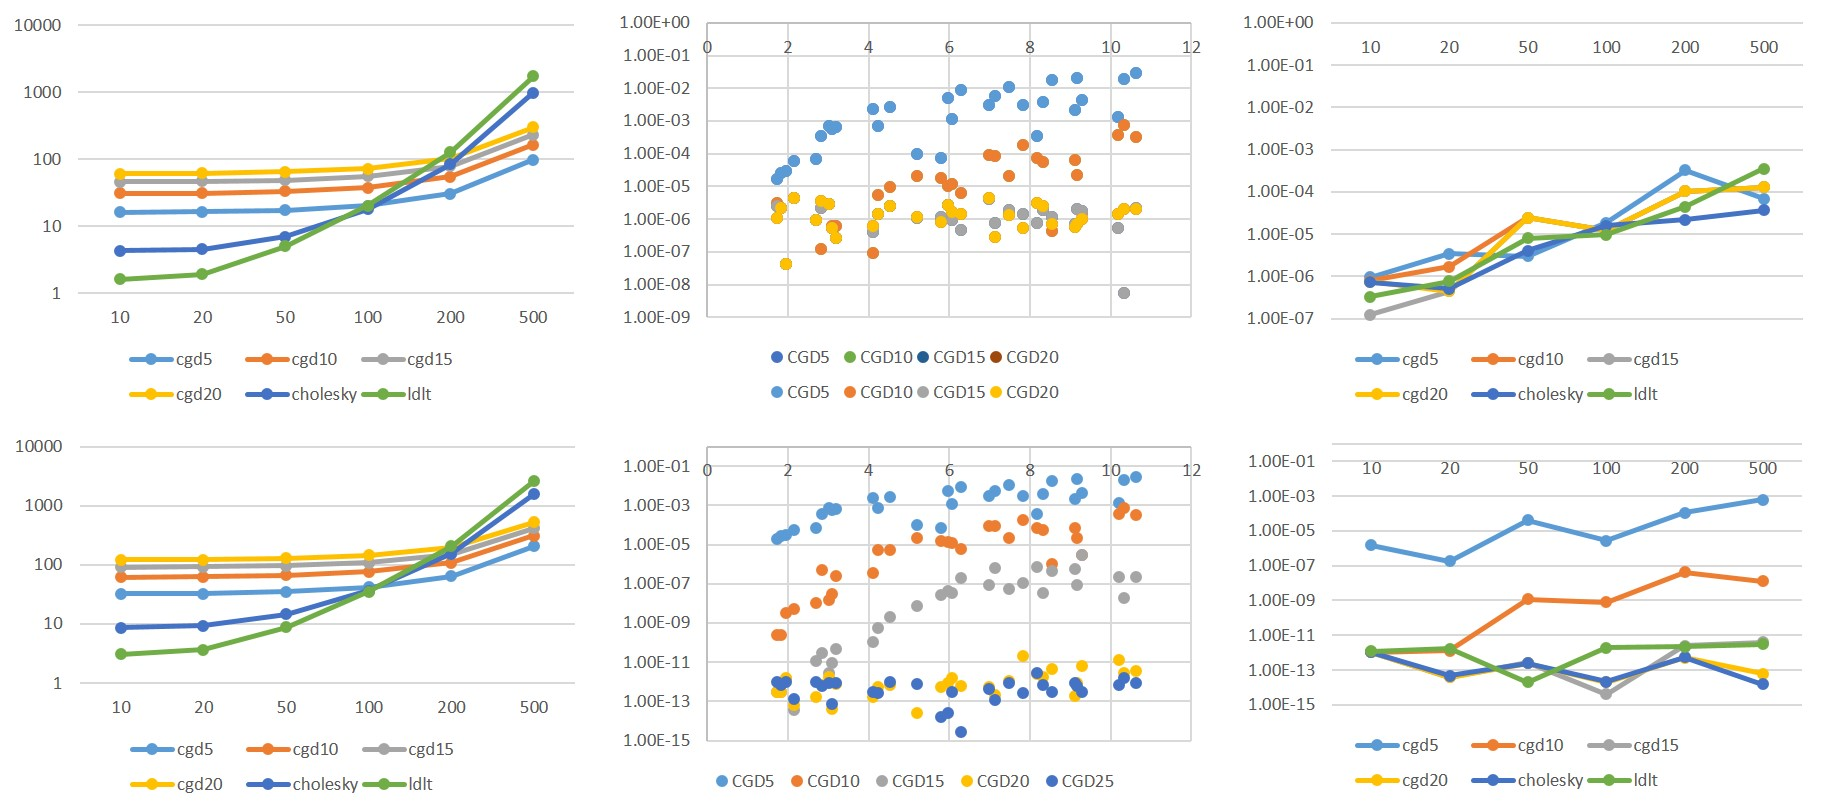
\includegraphics[width=\linewidth]{results.jpg}
  \caption{(Left) Comparison between different methods of solving linear systems: running time in seconds for Cholesky, LDLT, and CGD (with 5, 10, 15, and 20 iterations) as a function of input dimension. (Middle) Accuracy of CGD as a function of the input on the condition number of the input matrix A with d = 20. (Right) Accuracy of Cholesky, LDLT, and CGD, as a function of the input dimensionality d. (Top) Fixed-point numbers with the b = 80 bits, with 60 in the fractional part. (Bottom) b = 41, with 28 in the fractional part}
  \label{fig:result1}
\end{figure}

As expected, utilizing more bits gives much better accuracy. In both cases, the error results are comparable to the garbled circuits paper. However, we did find that the original experiment truncated the generated data at 12 decimal places, however we modified it so that we could work with the full representation of the number to get a better understanding of how accurate our algorithm is.  

The run times for SPDZ are always comparable if not much faster. In terms of run-time, we observe that both Cholesky and LDLT were faster for smaller dimensions when d $\leq$ 100 and CGD is faster for larger dimensions when d > 100. This is consistent with the findings in the original experiment. For dimensions 100 and smaller, when Cholesky and LDLT are faster, they comparative differences are not that big (LDLT with 1.6 seconds compared to CGD 20 with 60.89 seconds) when compared to the largest differences between the larger sizes (LDLT with 1747 seconds and CGD5 with 97 seconds).

[insert table comparison here??]

In the condition number experiment, for CGD iterations of 5, 10, and 15, error increases as condition number increases. For example, in CGD 10 a small condition number may have an error of 10e-9 yet a larger condition number could have an error as large as 10e-3. However, in the CGD 20 case, the condition number does not seem to have as much of effect as the range of errors is much less., with the error varying only form 10e-11 to 10e-14 keeping in mind these are much smaller increments. (why?? Add some explanation about how condition number affects errors in a matrix) For the 60 bit precision case, we chose to run more iterations because in the CGD 20 line, there is a noticeable upward slope in the scatter plot, indicating that still as condition numbers increased, the errors were increasing as well. Indeed, 25 iterations showed some improvement as we can see a flatter trend in the points. 

\end{document}









